\chapter{Theoretical Background \& Literature Survey}
\onehalfspacing

\section{Fundamentals of Sentiment Analysis}

Sentiment analysis --- also referred to as opinion mining --- is the computational discipline concerned with extracting, quantifying, and classifying subjective information from natural language \cite{liu2012sentiment}. What began as rule-based lexicon lookup in the early 2000s has evolved into a rich subfield of NLP that today encompasses document classification, aspect-level reasoning, emotion intensity regression, and cross-lingual transfer. Understanding this evolution is essential context for HinglishMSA, which inherits from two decades of methodological progress \cite{cambria2016affective}.

\subsection{Granularity Levels}

Sentiment analysis is applied at multiple levels of textual resolution. Each level poses a different modelling challenge and is suited to a different set of downstream applications.

\begin{table}[ht]
\centering
\caption{Granularity levels in sentiment analysis, with examples and typical NLP applications}
\label{tab:granularity}
\renewcommand{\arraystretch}{1.35}
\begin{tabular}{p{2.8cm} p{4.5cm} p{4.5cm}}
\toprule
\textbf{Level} & \textbf{Example} & \textbf{Application} \\
\midrule
Document-level   & Full product review rated positive & E-commerce brand monitoring \\
Sentence-level   & ``The camera is good but battery is terrible'' & News sentiment tracking \\
Aspect-level     & [camera: positive], [battery: negative] & Product comparison engines \\
Utterance-level  & Short spoken segment in a video clip & Video MSA (this work) \\
Token-level      & Per-word sentiment span tagging & Explanation generation \\
\bottomrule
\end{tabular}
\end{table}

Utterance-level analysis --- the level relevant to this thesis --- operates on short spoken or written segments that correspond to a single idea or opinion expression. Each clip in HinglishMSA is treated as one utterance with a single continuous sentiment score.

\subsection{Methodological Paradigms}

Wankhade et al. \cite{wankhade2022survey} and LeCun et al. \cite{lecun2015deep} collectively trace the evolution of SA methods through three paradigms, each representing a significant shift in how sentiment is operationalised. Figure~\ref{fig:sa_evolution} situates these paradigms on a chronological axis.

\begin{figure}[ht]
\centering
\begin{tikzpicture}[
    node distance=0.4cm and 0.1cm,
    era/.style={draw, fill=blue!8, minimum width=3.0cm, minimum height=1.6cm, align=center, font=\small},
    arr/.style={->, very thick, gray}
]
\node[era] (lex) {\textbf{Lexicon-Based}\\\scriptsize{1990s--2005}\\[3pt]\scriptsize SentiWordNet\\\scriptsize AFINN, OpinionFinder};
\node[era, right=0.55cm of lex] (ml) {\textbf{Traditional ML}\\\scriptsize{2005--2015}\\[3pt]\scriptsize SVM, Na\"ive Bayes\\\scriptsize n-gram features};
\node[era, right=0.55cm of ml] (dl) {\textbf{Deep Learning}\\\scriptsize{2015--2018}\\[3pt]\scriptsize LSTM, CNN\\\scriptsize Word2Vec, GloVe};
\node[era, right=0.55cm of dl] (tr) {\textbf{Transformers}\\\scriptsize{2018--present}\\[3pt]\scriptsize BERT, MuRIL\\\scriptsize LLM-assisted};
\draw[arr] (lex.east) -- (ml.west);
\draw[arr] (ml.east) -- (dl.west);
\draw[arr] (dl.east) -- (tr.west);
\end{tikzpicture}
\caption{Chronological evolution of sentiment analysis methodologies, from hand-crafted lexicons to pre-trained transformer models.}
\label{fig:sa_evolution}
\end{figure}

\textbf{Lexicon-based methods} assign polarity scores to individual words or phrases using curated dictionaries. The score for a document is typically an aggregation of its constituent word scores \cite{cambria2016affective}. While interpretable and requiring no training data, these methods collapse on domain-specific vocabulary, negation scopes, and code-mixed text where the sentiment lexicon covers only one of the two languages.

\textbf{Traditional machine learning} methods treat SA as a supervised classification problem. Features such as bag-of-words unigrams, bigrams, part-of-speech tags, and lexical patterns are fed to classifiers including Support Vector Machines (SVMs), Naive Bayes, and logistic regression \cite{wankhade2022survey}. The feature engineering bottleneck limits portability across languages and domains.

\textbf{Deep learning methods} remove the hand-crafting burden by learning hierarchical representations directly from data \cite{lecun2015deep}. Mikolov et al. \cite{mikolov2013distributed} showed that dense word representations (Word2Vec) trained on large corpora capture semantic relationships that dramatically improve downstream NLP tasks. Pennington et al. \cite{pennington2014glove} extended this with GloVe embeddings trained on global word co-occurrence statistics. Hochreiter and Schmidhuber's \cite{hochreiter1997lstm} Long Short-Term Memory (LSTM) networks became the default sequence encoder for sentiment throughout the 2015--2018 period, followed by the Transformer \cite{vaswani2017attention}.

\textbf{Transformer-based models} fine-tuned from BERT \cite{devlin2019bert} dominate modern benchmarks. The emergence of large language models (GPT-3 \cite{brown2020gpt3}, LLaMA \cite{touvron2023llama}) has further opened the possibility of zero-shot and few-shot SA using prompt engineering rather than labelled fine-tuning data.

\section{Multimodal Sentiment Analysis}

\subsection{Why Text Alone Is Not Enough}

A key observation motivating multimodal analysis is that lexical content alone is an incomplete carrier of sentiment \cite{poria2017review}. Consider the phrase ``Oh, really impressive.'' Delivered with an enthusiastic rising pitch and a genuine smile, the sentiment is unambiguously positive. Spoken slowly with flat intonation and a deadpan expression, it reads as sarcasm. The words are identical; the modality-level signals invert the meaning entirely. Poria et al. \cite{poria2017review} documented numerous such cases in their comprehensive review of affective computing, establishing empirically that audio and visual channels contribute non-redundant information to sentiment prediction.

Figure~\ref{fig:modality_features} illustrates the three modality streams and the representative features extracted from each in the HinglishMSA pipeline.

\begin{figure}[ht]
\centering
\begin{tikzpicture}[
    node distance=0.5cm and 0.8cm,
    head/.style={draw, fill=blue!12, minimum width=3.8cm, minimum height=0.72cm, align=center, font=\small\bfseries},
    feat/.style={draw, fill=gray!8, minimum width=3.8cm, minimum height=0.6cm, align=center, font=\scriptsize},
    arr/.style={->, thick}
]
% Column 1: Text
\node[head] (th) {Text (Linguistic)};
\node[feat, below=0.2cm of th] (t1) {Token embeddings};
\node[feat, below=0.15cm of t1] (t2) {Contextual [CLS] vector};
\node[feat, below=0.15cm of t2] (t3) {Sub-word morphology};
\node[feat, below=0.15cm of t3] (t4) {\textbf{MuRIL} $\rightarrow$ 768-dim};

% Column 2: Audio
\node[head, right=0.8cm of th] (ah) {Audio (Acoustic)};
\node[feat, below=0.2cm of ah] (a1) {Raw waveform (16\,kHz)};
\node[feat, below=0.15cm of a1] (a2) {Prosody, pitch, energy};
\node[feat, below=0.15cm of a2] (a3) {Phonetic patterns};
\node[feat, below=0.15cm of a3] (a4) {\textbf{wav2vec2-XLSR} $\rightarrow$ 1024-dim};

% Column 3: Visual
\node[head, right=0.8cm of ah] (vh) {Visual (Non-verbal)};
\node[feat, below=0.2cm of vh] (v1) {Video key frames};
\node[feat, below=0.15cm of v1] (v2) {Facial expressions};
\node[feat, below=0.15cm of v2] (v3) {Head pose, eye gaze};
\node[feat, below=0.15cm of v3] (v4) {\textbf{CLIP ViT-B/32} $\rightarrow$ 512-dim};

% Arrows
\draw[arr] (t3)--(t4); \draw[arr] (a3)--(a4); \draw[arr] (v3)--(v4);
\end{tikzpicture}
\caption{Three modality streams used in HinglishMSA and the feature representations extracted by the corresponding pre-trained encoders.}
\label{fig:modality_features}
\end{figure}

\subsection{Benchmark Datasets}

Zadeh et al. \cite{zadeh2016mosi} introduced CMU-MOSI, providing 2,199 opinion utterances from 93 YouTube monologue videos with continuous sentiment scores in $[-3, +3]$, annotated by five human workers using Amazon Mechanical Turk. CMU-MOSEI \cite{zadeh2018multimodal} extended the scope to 22,856 utterances from 3,228 YouTube videos spanning 250 distinct topics, making it the largest English MSA benchmark to date. The IEMOCAP dataset \cite{busso2008iemocap} provides 10,039 utterances from dyadic acted conversations with emotion and valence annotations, widely used for emotion recognition research. Table~\ref{tab:msa_datasets} compares these benchmarks.

\begin{table}[ht]
\centering
\caption{Comparison of major multimodal sentiment and emotion datasets}
\label{tab:msa_datasets}
\renewcommand{\arraystretch}{1.3}
\begin{tabular}{lcccccc}
\toprule
\textbf{Dataset} & \textbf{Language} & \textbf{Clips} & \textbf{Speakers} & \textbf{Annotation} & \textbf{Scale} & \textbf{Year} \\
\midrule
CMU-MOSI \cite{zadeh2016mosi}        & English  & 2{,}199  & 93   & Crowd   & $[-3,+3]$     & 2016 \\
CMU-MOSEI \cite{zadeh2018multimodal} & English  & 22{,}856 & 3{,}228 & Crowd & $[-3,+3]$     & 2018 \\
IEMOCAP \cite{busso2008iemocap}      & English  & 10{,}039 & 10   & Expert  & Categorical   & 2008 \\
MultiBench \cite{liang2021multibench} & English & varied   & --   & Mixed   & Multiple      & 2021 \\
\midrule
\textbf{HinglishMSA (ours)} & \textbf{Hinglish} & \textbf{2{,}652} & \textbf{1{,}174} & \textbf{LLM} & $\mathbf{[-3,+3]}$ & \textbf{2026} \\
\bottomrule
\end{tabular}
\end{table}

\subsection{Multimodal Fusion Strategies}

Three broad strategies exist for combining information from multiple modalities \cite{guo2023recent}. Figure~\ref{fig:fusion_strategies} contrasts their structural differences.

\begin{figure}[ht]
\centering
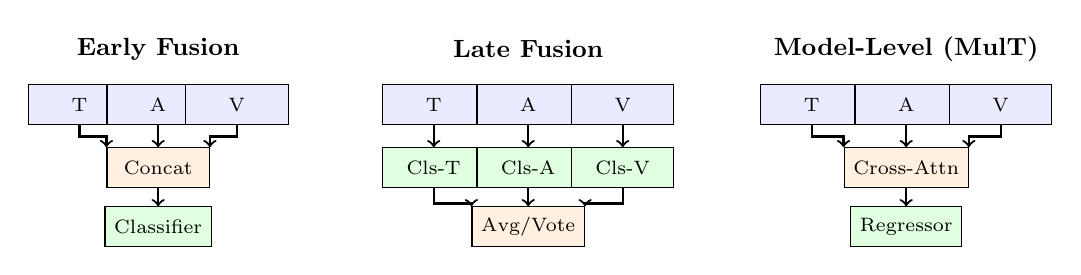
\begin{tikzpicture}[
    node distance=0.35cm,
    mod/.style={draw, fill=blue!8, minimum width=1.3cm, minimum height=0.5cm, align=center, font=\scriptsize},
    fus/.style={draw, fill=orange!12, minimum width=1.3cm, minimum height=0.5cm, align=center, font=\scriptsize},
    cls/.style={draw, fill=green!12, minimum width=1.3cm, minimum height=0.5cm, align=center, font=\scriptsize},
    arr/.style={->, thick},
    lbl/.style={font=\small\bfseries, align=center}
]
% --- Early Fusion ---
\node[lbl] at (1.5, 0.3) {Early Fusion};
\node[mod] (et) at (0.5, -0.4) {T};
\node[mod] (ea) at (1.5, -0.4) {A};
\node[mod] (ev) at (2.5, -0.4) {V};
\node[fus] (ec) at (1.5, -1.2) {Concat};
\node[cls] (eo) at (1.5, -1.95) {Classifier};
\draw[arr] (et.south) -- ++(0,-0.15) -| (ec.north west);
\draw[arr] (ea)--(ec);
\draw[arr] (ev.south) -- ++(0,-0.15) -| (ec.north east);
\draw[arr] (ec)--(eo);

% --- Late Fusion ---
\node[lbl] at (6.2, 0.3) {Late Fusion};
\node[mod] (lt) at (5.0, -0.4) {T};
\node[mod] (la) at (6.2, -0.4) {A};
\node[mod] (lv) at (7.4, -0.4) {V};
\node[cls] (lct) at (5.0, -1.2) {Cls-T};
\node[cls] (lca) at (6.2, -1.2) {Cls-A};
\node[cls] (lcv) at (7.4, -1.2) {Cls-V};
\node[fus] (lc) at (6.2, -1.95) {Avg/Vote};
\draw[arr] (lt)--(lct); \draw[arr] (la)--(lca); \draw[arr] (lv)--(lcv);
\draw[arr] (lct.south) -- ++(0,-0.2) -| (lc.north west);
\draw[arr] (lca)--(lc);
\draw[arr] (lcv.south) -- ++(0,-0.2) -| (lc.north east);

% --- Model-Level ---
\node[lbl] at (11.0, 0.3) {Model-Level (MulT)};
\node[mod] (mt) at (9.8, -0.4) {T};
\node[mod] (ma) at (11.0, -0.4) {A};
\node[mod] (mv) at (12.2, -0.4) {V};
\node[fus] (mc) at (11.0, -1.2) {Cross-Attn};
\node[cls] (mo) at (11.0, -1.95) {Regressor};
\draw[arr] (mt.south) -- ++(0,-0.15) -| (mc.north west);
\draw[arr] (ma)--(mc);
\draw[arr] (mv.south) -- ++(0,-0.15) -| (mc.north east);
\draw[arr] (mc)--(mo);
\end{tikzpicture}
\caption{Three multimodal fusion strategies. Early fusion concatenates raw features; late fusion combines independent unimodal predictions; model-level fusion (used in this thesis via MulT) learns cross-modal interactions during representation learning.}
\label{fig:fusion_strategies}
\end{figure}

\textbf{Early fusion} simply concatenates the feature vectors from all modalities before passing them to a classifier. While conceptually simple, it is sensitive to differences in temporal resolution and feature scale across modalities. \textbf{Late fusion} trains independent unimodal models and combines their predictions via averaging or voting, losing the opportunity to learn cross-modal correlations. \textbf{Model-level (hybrid) fusion} integrates the modalities during the representation learning process itself, enabling each modality to inform the representation of the others \cite{tsai2019multimodal}. Pham et al. \cite{pham2019found} extended this idea using cyclic translation losses; Hazarika et al. \cite{hazarika2020misa} factorised representations into modality-invariant and modality-specific components; Yang et al. \cite{yang2021mtag} introduced modal-temporal attention graphs for unaligned sequences.

\section{Attention Mechanisms and Transformer Architecture}

\subsection{Scaled Dot-Product Attention}

The attention mechanism introduced by Vaswani et al. \cite{vaswani2017attention} is the central computational primitive of modern NLP. Given a sequence of query vectors $Q \in \mathbb{R}^{n \times d_k}$, key vectors $K \in \mathbb{R}^{m \times d_k}$, and value vectors $V \in \mathbb{R}^{m \times d_v}$, the scaled dot-product attention computes:

\begin{equation}
\text{Attention}(Q, K, V) = \text{softmax}\left(\frac{QK^\top}{\sqrt{d_k}}\right) V
\label{eq:attention}
\end{equation}

The $\sqrt{d_k}$ scaling prevents the dot products from growing large in magnitude as $d_k$ increases, which would push the softmax into regions of extremely small gradients. Multi-head attention runs $h$ parallel attention heads with different learned projections:

\begin{equation}
\text{MultiHead}(Q, K, V) = \text{Concat}(\text{head}_1, \ldots, \text{head}_h)\,W^O
\label{eq:multihead}
\end{equation}

where $\text{head}_i = \text{Attention}(QW_i^Q,\, KW_i^K,\, VW_i^V)$ and $W_i^Q \in \mathbb{R}^{d_{\text{model}} \times d_k}$, $W_i^K \in \mathbb{R}^{d_{\text{model}} \times d_k}$, $W_i^V \in \mathbb{R}^{d_{\text{model}} \times d_v}$, $W^O \in \mathbb{R}^{hd_v \times d_{\text{model}}}$.

A Transformer encoder block stacks multi-head self-attention with a position-wise feed-forward network (FFN) and layer normalisation \cite{vaswani2017attention}:
\begin{align}
\mathbf{z} &= \text{LayerNorm}\left(\mathbf{x} + \text{MultiHead}(\mathbf{x}, \mathbf{x}, \mathbf{x})\right) \label{eq:ln1}\\
\mathbf{y} &= \text{LayerNorm}\left(\mathbf{z} + \text{FFN}(\mathbf{z})\right) \label{eq:ln2}
\end{align}
where $\text{FFN}(\mathbf{z}) = \max(0, \mathbf{z}W_1 + b_1)W_2 + b_2$ is a two-layer MLP with ReLU activation.

\subsection{Cross-Modal Attention in MulT}

The Multimodal Transformer (MulT) \cite{tsai2019multimodal} generalises self-attention to the cross-modal setting. In cross-modal attention from modality $\beta$ to modality $\alpha$, the query vectors are projected from $\alpha$ while the keys and values come from $\beta$:

\begin{equation}
Z_{\alpha \leftarrow \beta} = \text{CM-Attn}(Z_\alpha, Z_\beta) = \text{softmax}\left(\frac{(Z_\alpha W_\alpha^Q)(Z_\beta W_\beta^K)^\top}{\sqrt{d_k}}\right)(Z_\beta W_\beta^V)
\label{eq:cross_attn}
\end{equation}

Equation~\ref{eq:cross_attn} allows modality $\alpha$ to query information from modality $\beta$ at any time step, regardless of temporal alignment. Figure~\ref{fig:ch2crossattn} illustrates this directional flow for the three-modality case.

\begin{figure}[ht]
\centering
\begin{tikzpicture}[
    node distance=0.5cm and 1.0cm,
    mod/.style={draw, fill=blue!10, minimum width=2.0cm, minimum height=0.65cm, align=center, font=\small\bfseries},
    attn/.style={draw, fill=orange!15, minimum width=2.0cm, minimum height=0.55cm, align=center, font=\scriptsize},
    fused/.style={draw, fill=green!10, minimum width=2.0cm, minimum height=0.55cm, align=center, font=\scriptsize},
    arr/.style={->, thick},
    darr/.style={->, thick, dashed, gray}
]
\node[mod] (T) {Text ($Z_T$)};
\node[mod, right=1.0cm of T] (A) {Audio ($Z_A$)};
\node[mod, right=1.0cm of A] (V) {Visual ($Z_V$)};

\node[attn, below=1.0cm of T] (atT) {$Z_{T\leftarrow A}$, $Z_{T\leftarrow V}$};
\node[attn, below=1.0cm of A] (atA) {$Z_{A\leftarrow T}$, $Z_{A\leftarrow V}$};
\node[attn, below=1.0cm of V] (atV) {$Z_{V\leftarrow T}$, $Z_{V\leftarrow A}$};

\node[fused, below=0.6cm of atT] (fT) {Fused $\hat{Z}_T$};
\node[fused, below=0.6cm of atA] (fA) {Fused $\hat{Z}_A$};
\node[fused, below=0.6cm of atV] (fV) {Fused $\hat{Z}_V$};

% Self arrows (Q source)
\draw[arr] (T)--(atT);
\draw[arr] (A)--(atA);
\draw[arr] (V)--(atV);

% Cross arrows (K,V source): A,V -> T block
\draw[darr] (A.south) -- ++(0,-0.3) -| (atT.north east);
\draw[darr] (V.south) -- ++(0,-0.4) -| (atT.east);

% Cross arrows: T,V -> A block
\draw[darr] (T.south) -- ++(0,-0.3) -| (atA.north west);
\draw[darr] (V.south) -- ++(0,-0.3) -| (atA.north east);

% Cross arrows: T,A -> V block
\draw[darr] (T.south) -- ++(0,-0.4) -| (atV.west);
\draw[darr] (A.south) -- ++(0,-0.3) -| (atV.north west);

\draw[arr] (atT)--(fT); \draw[arr] (atA)--(fA); \draw[arr] (atV)--(fV);
\end{tikzpicture}
\caption{Cross-modal attention in MulT. Solid arrows indicate the query source (the modality being enriched); dashed arrows indicate key-value sources (the modalities providing context). Each fused representation $\hat{Z}_\alpha$ integrates attended information from both other modalities.}
\label{fig:ch2crossattn}
\end{figure}

\subsection{Evaluation Metrics}

This thesis adopts the standard evaluation protocol from CMU-MOSI \cite{zadeh2016mosi}. Let $\hat{y}_i$ denote the predicted sentiment score and $y_i$ the ground-truth label for the $i$-th sample. The following metrics are reported:

\begin{align}
\text{MAE} &= \frac{1}{N}\sum_{i=1}^{N}\lvert y_i - \hat{y}_i \rvert \label{eq:mae}\\[4pt]
r &= \frac{\sum_i (y_i - \bar{y})(\hat{y}_i - \bar{\hat{y}})}{\sqrt{\sum_i (y_i-\bar{y})^2 \sum_i (\hat{y}_i - \bar{\hat{y}})^2}} \label{eq:pearson}\\[4pt]
\text{Acc}_2 &= \frac{1}{N}\sum_{i=1}^{N}\mathbf{1}[\text{sign}(\hat{y}_i) = \text{sign}(y_i)] \label{eq:acc2}\\[4pt]
F_1 &= \frac{2 \cdot \text{Precision} \cdot \text{Recall}}{\text{Precision} + \text{Recall}} \label{eq:f1}
\end{align}

Lower MAE (Eq.~\ref{eq:mae}) and higher Pearson correlation $r$ (Eq.~\ref{eq:pearson}) indicate better regression performance. Binary accuracy $\text{Acc}_2$ (Eq.~\ref{eq:acc2}) and $F_1$ (Eq.~\ref{eq:f1}) measure performance on the coarser but practically relevant positive-vs-negative classification task. The model is trained with mean squared error (MSE) loss: $\mathcal{L} = \frac{1}{N}\sum_{i=1}^{N}(y_i - \hat{y}_i)^2$.

\section{Code-Mixed Language Processing}

\subsection{Linguistic Phenomena}

Code-mixing and code-switching describe the alternation between two or more languages within a discourse, a sentence, or even a single morpheme \cite{barman2014code}. Srinivasan and Subalalitha \cite{srinivasan2020code} define three structural categories:

\begin{itemize}
    \item \textbf{Inter-sentential switching:} The language changes at sentence boundaries. This is the structurally simplest form and is handled adequately by most multilingual models.
    \item \textbf{Intra-sentential mixing:} Languages are interleaved within a single sentence. This is the dominant mode in Hinglish: ``\textit{Mujhe yeh presentation bahut helpful lagi}'' (I found this presentation very helpful). Standard monolingual models fail on such utterances.
    \item \textbf{Tag switching:} A tag or filler from one language is inserted into an utterance in another, e.g., appending ``\textit{yaar}'' (friend) or ``\textit{na}'' (emphasis) to otherwise English sentences.
\end{itemize}

Code-mixing is not linguistically arbitrary. Myers-Scotton's Matrix Language Frame model predicts that one language provides the morphosyntactic frame (the matrix language) while content items from the other (the embedded language) are inserted at specific constituent boundaries. In Hinglish, Hindi typically serves as the matrix language for spoken content, while English provides nouns, verbs, and technical vocabulary \cite{srinivasan2020code}.

\subsection{Challenges for NLP Systems}

Handling Hinglish text computationally presents a cascade of compounding difficulties:

\begin{enumerate}
    \item \textbf{Language identification:} Standard language identification tools (LangDetect, FastText's LID) assign a single language label to each text segment. Hinglish utterances receive inconsistent labels --- sometimes classified as Hindi, sometimes as English, often as an unrecognised language \cite{aguilar2020lince, barman2014code}.

    \item \textbf{Tokenisation:} BERT-family models use subword tokenisation (WordPiece or BPE) trained on monolingual corpora. Hinglish words that do not appear in either the Hindi or English vocabulary are aggressively split into character-level pieces or mapped to \texttt{[UNK]}, discarding lexical information.

    \item \textbf{ASR transcription quality:} Speech recognition systems trained on a single language produce high error rates on code-switched input. A Whisper model trained on Hindi will substitute English words with phonetically similar Hindi alternatives; the reverse holds for English-trained models \cite{radford2023whisper}.

    \item \textbf{Transliteration variation:} Hinglish is commonly written in Romanised form (Latin script) with no standardised spelling. The same Hindi word may appear as ``\textit{kya}'', ``\textit{kia}'', or ``\textit{kyaa}'' across different speakers \cite{winata2019code}.

    \item \textbf{Data scarcity:} Annotated Hinglish datasets are small, domain-specific, and limited to text modality \cite{joshi2016towards}. No multimodal resource existed prior to this work.
\end{enumerate}

\subsection{Existing Hinglish and Code-Mixed Resources}

Table~\ref{tab:codemix_datasets} surveys prior work on code-mixed NLP resources, revealing the data gap that HinglishMSA fills.

\begin{table}[ht]
\centering
\caption{Existing code-mixed NLP datasets, predominantly text-only and small-scale}
\label{tab:codemix_datasets}
\renewcommand{\arraystretch}{1.3}
\begin{tabular}{p{3.5cm} p{2.5cm} p{1.8cm} p{1.6cm} p{2.5cm}}
\toprule
\textbf{Dataset / Work} & \textbf{Language Pair} & \textbf{Size} & \textbf{Modality} & \textbf{Task} \\
\midrule
Joshi et al.\ \cite{joshi2016towards}      & Hindi-English & 3{,}879 & Text & Sentiment \\
Barman et al.\ \cite{barman2014code}       & English-Bengali & 1{,}239 & Text & LID \\
LinCE \cite{aguilar2020lince}              & Multiple pairs & varied  & Text & Multi-task \\
Winata et al.\ \cite{winata2019code}       & Multiple pairs & varied  & Text & LM \\
\midrule
\textbf{HinglishMSA (ours)} & \textbf{Hindi-English} & \textbf{2{,}652} & \textbf{T+A+V} & \textbf{Sentiment} \\
\bottomrule
\end{tabular}
\end{table}

HinglishMSA is the first entry in this table to provide multimodal (text, audio, and visual) annotation for a code-mixed Indian language pair.

\section{Pre-trained Foundation Models}

\subsection{BERT and the Rise of Contextual Representations}

Devlin et al. \cite{devlin2019bert} introduced BERT (Bidirectional Encoder Representations from Transformers), trained on masked language modelling (MLM) and next-sentence prediction (NSP) objectives over 3.3 billion tokens of English text. BERT's key innovation is bidirectionality: unlike previous left-to-right language models, BERT's representations are conditioned on both left and right context simultaneously, producing richer, more context-sensitive embeddings. Fine-tuning BERT on downstream tasks yields state-of-the-art performance across the GLUE benchmark with minimal task-specific architecture changes.

Multilingual BERT (mBERT) extends the same pre-training to 104 languages using a shared 110,000-token subword vocabulary. Zero-shot cross-lingual transfer to unseen languages is possible in some settings, but performance degrades significantly for typologically distant language pairs. For Indian languages in particular, the small proportion of Indic text in mBERT's training corpus means that Hindi representations are substantially weaker than those for European languages \cite{khanuja2021muril}.

\subsection{MuRIL: Tailored for Indian Languages}

Khanuja et al. \cite{khanuja2021muril} developed MuRIL (Multilingual Representations for Indian Languages) by pre-training a BERT-architecture model on 17 Indian languages plus their transliterated forms, sourcing text from Wikipedia, Common Crawl, DailyHunt, and online forums that contain naturally occurring code-mixed content. MuRIL's training data explicitly includes Hindi-English code-mixed text, making it the most appropriate text encoder for Hinglish downstream tasks.

MuRIL operates on a 197,000-token sentencepiece vocabulary that covers Devanagari, Latin script, and transliteration variants of all 17 supported languages. In this thesis, the \texttt{google/muril-base-cased} checkpoint produces 768-dimensional [CLS] token embeddings that serve as the text representation for each Hinglish clip. MuRIL has been shown to outperform mBERT by a substantial margin on named entity recognition, part-of-speech tagging, and question answering in Hindi and related languages.

\subsection{wav2vec 2.0 and XLSR-53}

Baevski et al. \cite{baevski2020wav2vec} introduced wav2vec 2.0, a self-supervised framework for learning representations directly from raw audio waveforms. The model architecture comprises three components: (1) a multi-layer convolutional feature encoder that maps raw waveform to a sequence of latent speech representations; (2) a quantisation module that discretises these representations into a finite codebook; and (3) a Transformer context network that produces contextualized representations using masked prediction over the quantised targets. The contrastive objective encourages the context representation at a masked time step to be closer to the true quantised representation than to distractors. Formally:

\begin{equation}
\mathcal{L}_\text{wav2vec} = -\log \frac{\exp(\text{sim}(c_t, q_t)/\kappa)}{\sum_{\tilde{q} \in Q_t}\exp(\text{sim}(c_t,\tilde{q})/\kappa)}
\label{eq:wav2vec}
\end{equation}

where $c_t$ is the context representation, $q_t$ is the true quantised target, $\tilde{q}$ are distractors, $\text{sim}(\cdot, \cdot)$ is cosine similarity, and $\kappa$ is a temperature parameter.

Conneau et al. \cite{conneau2021xlsr} trained XLSR-53 by extending wav2vec 2.0 to 53 languages, using a shared quantised vocabulary across all languages. The multi-language training creates a joint phonetic-acoustic space that enables cross-lingual speech transfer. In this thesis, \texttt{facebook/wav2vec2-large-xlsr-53} produces 1024-dimensional mean-pooled representations from Hinglish audio, capturing vocal affect cues (stress patterns, intonation contours, speech rate) in a language-agnostic embedding space.

\subsection{CLIP: Contrastive Language-Image Pre-training}

Radford et al. \cite{radford2021clip} trained CLIP on 400 million image-text pairs sourced from the internet, using a symmetric contrastive objective that aligns visual and textual representations:

\begin{equation}
\mathcal{L}_\text{CLIP} = -\frac{1}{2}\left[\log\frac{\exp(\langle f_I, f_T \rangle/\tau)}{\sum_j \exp(\langle f_I, f_{T_j} \rangle/\tau)} + \log\frac{\exp(\langle f_T, f_I \rangle/\tau)}{\sum_j \exp(\langle f_{T_j}, f_I \rangle/\tau)}\right]
\label{eq:clip}
\end{equation}

where $f_I$ and $f_T$ denote the image and text embeddings, and $\tau$ is a learnable temperature. The ViT-B/32 visual encoder tokenises a $224\times 224$ image into $14\times 14 = 196$ patches of $16\times 16$ pixels each, processes them through a 12-layer Vision Transformer, and outputs a 512-dimensional [CLS] representation. In HinglishMSA, five key frames are extracted per video clip and CLIP embeddings are averaged to form a single 512-dimensional visual representation per clip.

\subsection{Whisper: Robust Multilingual ASR}

Radford et al. \cite{radford2023whisper} trained Whisper on 680,000 hours of multilingual audio in a weakly supervised sequence-to-sequence framework, using a standard cross-entropy objective over predicted transcript tokens. The \texttt{large-v3} model contains 1.55 billion parameters and achieves near-human error rates on English, with strong performance across the 99 supported languages including Hindi. In this thesis, faster-whisper (a CTranslate2-based inference engine for Whisper) is used to transcribe 50,695 candidate audio clips at float16 precision with CUDA acceleration.

\subsection{Comparison of Encoders Used in This Thesis}

\begin{table}[ht]
\centering
\caption{Pre-trained encoders used in MulTHinglish: architecture, output dimensionality, and language coverage}
\label{tab:encoders}
\renewcommand{\arraystretch}{1.3}
\begin{tabular}{lllll}
\toprule
\textbf{Model} & \textbf{Modality} & \textbf{Arch.} & \textbf{Dim} & \textbf{Languages} \\
\midrule
MuRIL-base \cite{khanuja2021muril}          & Text   & BERT-base   & 768   & 17 Indian langs + transliteration \\
wav2vec2-XLSR-53 \cite{conneau2021xlsr}     & Audio  & Transformer & 1024  & 53 languages \\
CLIP ViT-B/32 \cite{radford2021clip}        & Visual & ViT         & 512   & Language-agnostic \\
Whisper large-v3 \cite{radford2023whisper}  & ASR    & Seq2Seq     & --    & 99 languages \\
\bottomrule
\end{tabular}
\end{table}

\section{Large Language Models for Annotation}

The emergence of large language models capable of understanding nuanced sentiment has opened a compelling avenue for automated dataset annotation. Brown et al. \cite{brown2020gpt3} demonstrated that GPT-3 (175 billion parameters) can perform few-shot sentiment classification with no task-specific fine-tuning, simply from in-context examples. Touvron et al. \cite{touvron2023llama} later showed that open-source models at the LLaMA family scales (7B--65B parameters) can match or exceed GPT-3's capabilities on many benchmarks while being deployable without proprietary API access.

In HinglishMSA, the Groq inference API provides sub-second latency access to \texttt{llama\allowbreak-3.1\allowbreak-8b\allowbreak-instant}, enabling annotation of 2,652 clips in approximately two hours. The annotation prompt provides each clip's transcription and requests a sentiment score in $[-3, +3]$ along with a brief justification. Confidence stratification is derived from the absolute magnitude of the predicted score: clips with $|s| > 1.5$ are considered high-confidence, while clips with $|s| \leq 0.5$ are flagged as low-confidence. This scheme draws on the intuition that strong unambiguous sentiments (clearly positive or clearly negative) are more reliably annotated by an LLM than ambiguous neutral-leaning utterances.

The validity of LLM-based annotation for sentiment has been examined by several recent studies. While LLM annotations do not perfectly replicate human judgements, they exhibit acceptable inter-rater agreement for binary sentiment classification and provide consistent scores across repeated runs \cite{touvron2023llama}. For under-resourced languages where crowdsourcing is impractical, LLM annotation represents a tractable and scalable alternative.

\section{Summary and Research Gap}

Table~\ref{tab:litsurvey} provides a structured summary of the key prior works surveyed in this chapter and their relationship to the contributions of this thesis.

\begin{table}[ht]
\centering
\caption{Summary of directly relevant prior works and their contribution to this thesis}
\label{tab:litsurvey}
\renewcommand{\arraystretch}{1.3}
\begin{tabular}{p{3.2cm} p{3.0cm} p{2.0cm} p{4.0cm}}
\toprule
\textbf{Work} & \textbf{Focus} & \textbf{Modality} & \textbf{Relevance to this thesis} \\
\midrule
Liu \cite{liu2012sentiment}                & SA fundamentals    & Text    & Conceptual foundation \\
Zadeh et al.\ \cite{zadeh2016mosi}         & CMU-MOSI dataset   & T+A+V   & Evaluation protocol, baseline \\
Zadeh et al.\ \cite{zadeh2018multimodal}   & CMU-MOSEI dataset  & T+A+V   & Extended MSA benchmark \\
Tsai et al.\ \cite{tsai2019multimodal}     & MulT architecture  & T+A+V   & Core model design \\
Vaswani et al.\ \cite{vaswani2017attention}& Transformer        & --      & Attention mechanism \\
Hazarika et al.\ \cite{hazarika2020misa}   & MISA fusion        & T+A+V   & Fusion design context \\
Yang et al.\ \cite{yang2021mtag}           & MTAG               & T+A+V   & Fusion design context \\
Khanuja et al.\ \cite{khanuja2021muril}    & MuRIL              & Text    & Text encoder \\
Conneau et al.\ \cite{conneau2021xlsr}     & XLSR-53            & Audio   & Audio encoder \\
Radford et al.\ \cite{radford2021clip}     & CLIP               & Visual  & Visual encoder \\
Radford et al.\ \cite{radford2023whisper}  & Whisper            & Audio   & ASR pipeline \\
Joshi et al.\ \cite{joshi2016towards}      & Hinglish SA        & Text    & Code-mixed NLP background \\
Barman et al.\ \cite{barman2014code}       & Code-mix LID       & Text    & Language ID challenges \\
Aguilar et al.\ \cite{aguilar2020lince}    & LinCE benchmark    & Text    & Code-switch evaluation \\
Touvron et al.\ \cite{touvron2023llama}    & LLaMA LLM          & Text    & Annotation pipeline \\
\bottomrule
\end{tabular}
\end{table} 

The survey reveals a clear and multi-dimensional research gap. On the data side, every multimodal sentiment benchmark is English-only, while every Hinglish NLP resource is text-only and small-scale. On the model side, English-centric encoders fail to represent code-mixed Hinglish semantics, and no prior work has combined cross-lingual multilingual encoders in a unified multimodal sentiment framework. On the annotation side, scalable approaches to labelling under-resourced code-mixed video content have not been demonstrated.

This thesis addresses all three dimensions simultaneously: constructing the HinglishMSA dataset, proposing the MulTHinglish model, and demonstrating the viability of LLM-assisted annotation for code-mixed multimodal content. Each contribution closes a specific gap documented in this chapter, and together they establish the first complete pipeline for Hinglish multimodal sentiment analysis.

\newpage